\section{The navigator}
\label{sec:navigator}
A navigator must comply with some requirements to create a huge metaverse and democratize its use. First of all, the Ogre 3D rendering engine have been choosed for its robustness, efficiency, upgradability and openess that are necessary for a durable system. Moreover, Ogre 3D can be easily embedded in web pages thanks to a mozilla plugin or a ActiveX. Conversely, web pages can be mapped on 3D models as interactive textures thanks to the Navi library based on Gecko. Thus, the navigator allows a Web 2.0 navigation inside the Web 3D, as well as a Web 3D navigation inside the Web 2.0, as we clearly think that web 3D and web 2.0 are additional (see figure \ref{Fig:navigator}). 
\begin{figure}
\center
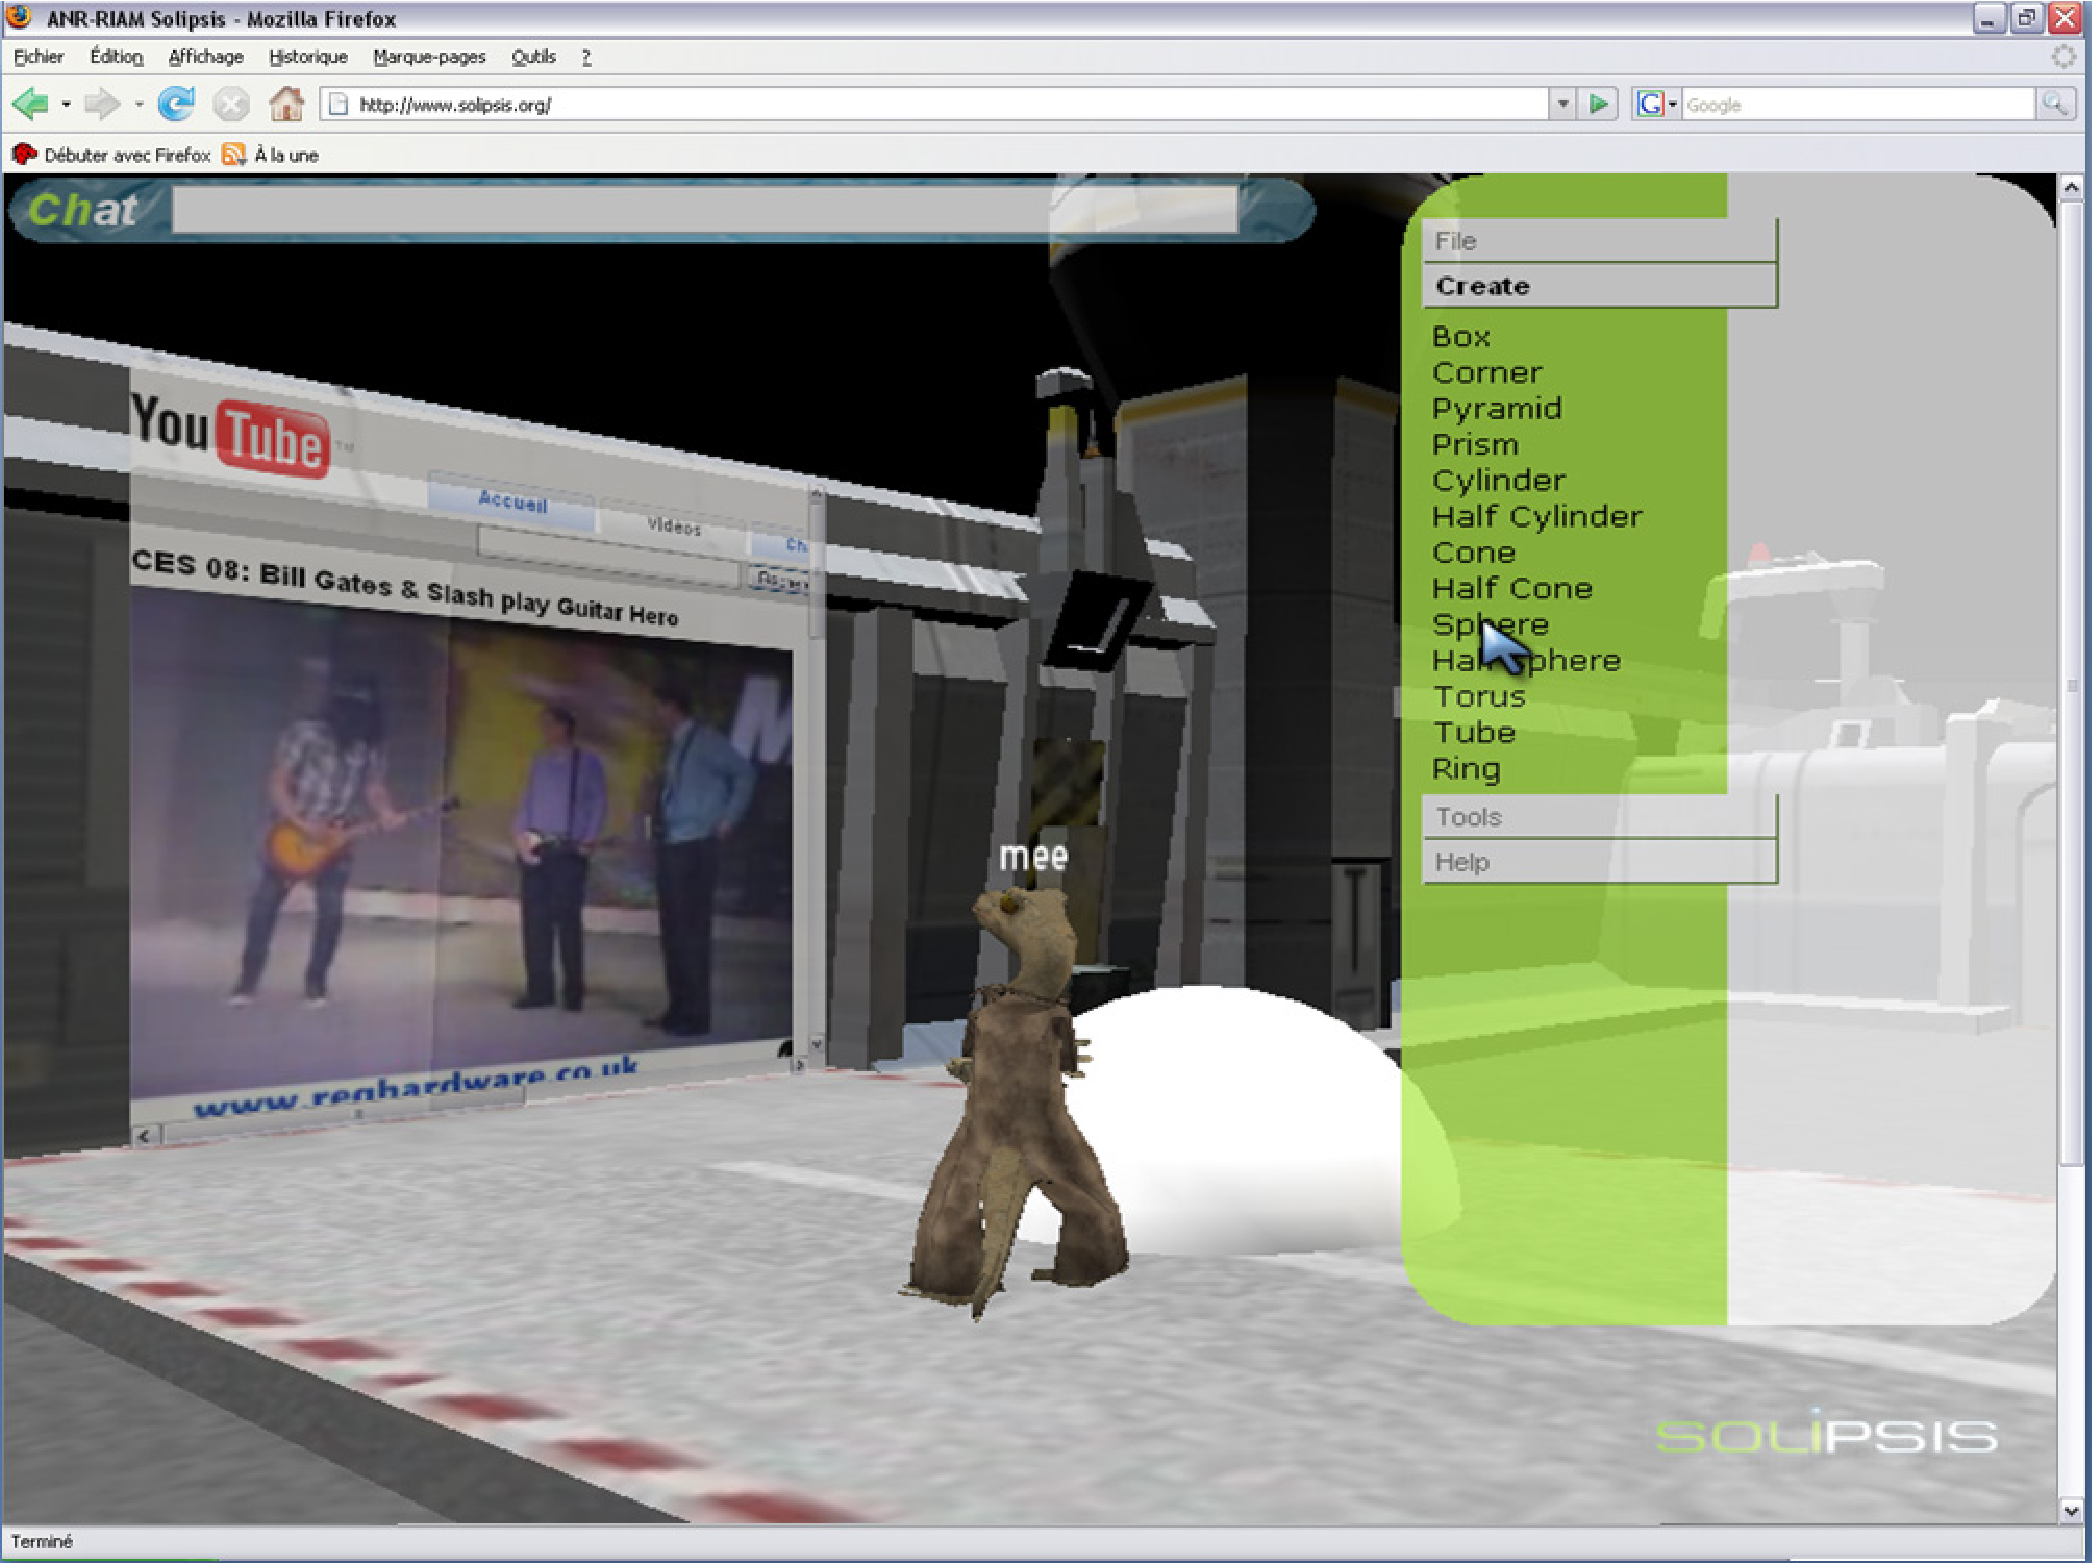
\includegraphics[width=3in]{Figures/navigator.pdf}
\caption{Web based navigator embedding modeling tools, and providing a mapping of web pages as interactive textures.}
\label{Fig:navigator}
\end{figure}
Since the vitual universe belongs to all users, modeling tools are embedded within the navigator in order to create, modify or delete contents. At the moment, we focus on intuitive tools, but procedural, declartive, parametric and sketching based modeling tools are obviously considered. Finally, to provide accesses to the virtual universe in mobility, nodes can be hosted by proxy servers, to reduce the amount of processes that have to be executed on terminals with low ressources. Thus, hosts can compute detection collision, physic animation, data exchange management, viewpoint based filtering, and communicate with the navigator that has just to render the virtual environment and interact with it (see figure \ref{Fig:host}).
\begin{figure}
\center
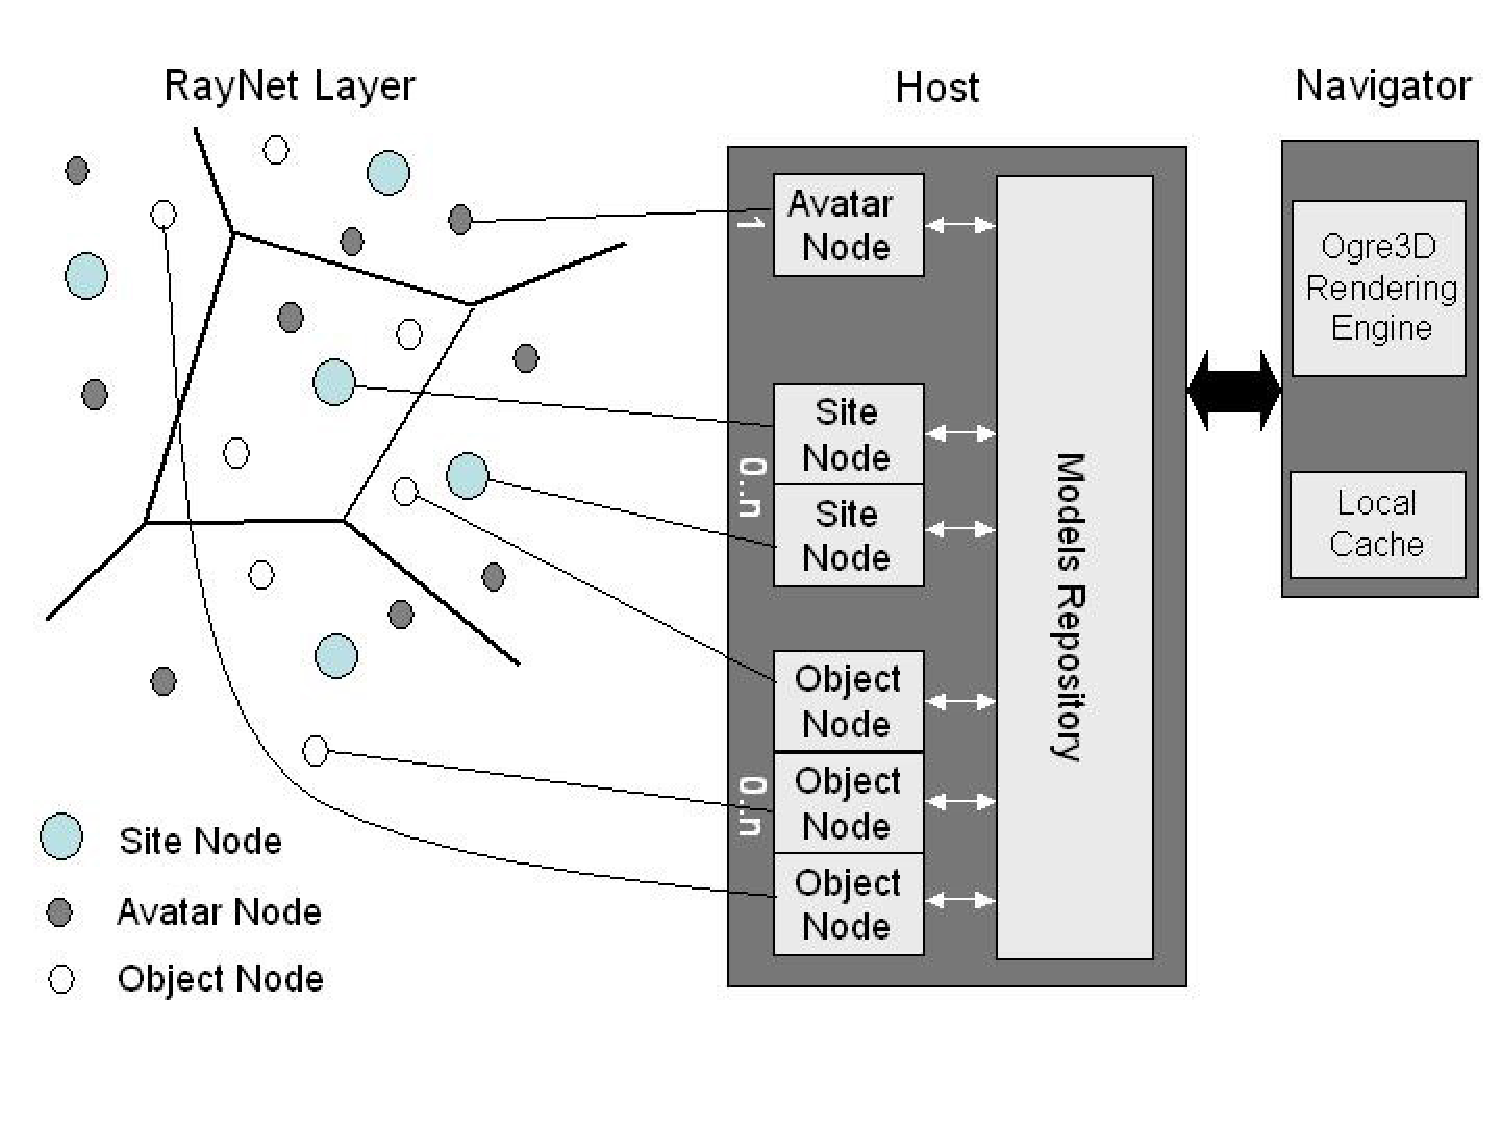
\includegraphics[width=3in]{Figures/host.pdf}
\caption{Nodes hosted on a proxy server to allow accesses to the metaverse on terminals with low ressources such as mobiles.}
\label{Fig:host}
\end{figure}